% !TeX root = ../dd.tex

\section{Architectural Design}

\subsection{Overview}
% High-level component and their interaction
To ensure high maintainability, scalability and security, the service is structured according to the well-established three-tier architecture.
Figure \ref{fig:overview-architecture} shows how the tiers are divided, and what are the relations between key components of the system.

\begin{figure}[H]
    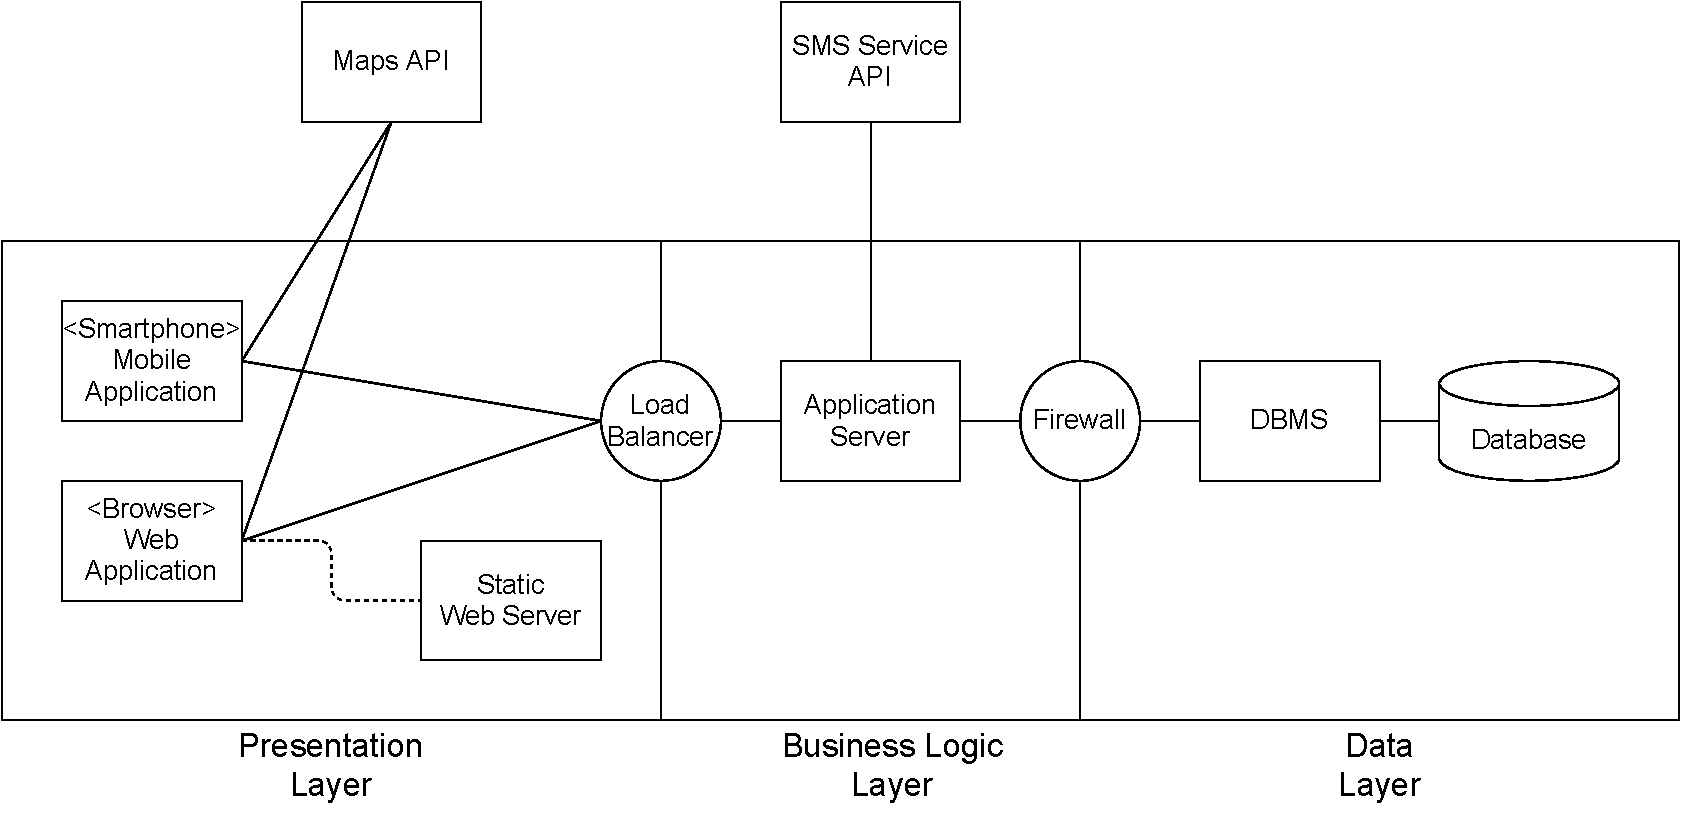
\includegraphics[width=\linewidth]{images/draw.io/overview_architecture.pdf}
    \caption{Overall architecture of the System}
    \label{fig:overview-architecture}
\end{figure}

The main components are the following:

\begin{itemize}
    \item \textbf{Mobile Application} The application is installed on the user's device through its store platform service. The application allows the user to interact with the service and receive notifications from the server.
    \item \textbf{Web Application} The web application allows users to access the same services available on the mobile app through any device, but it's not guaranteed that it can receive notifications. In addition to that, store managers may access a dedicated panel to configure additional parameters.
    \item \textbf{Static Web Server} It serves the client's browser a bundle that contains the web application code (compressed HTML and JS). It has no ties with the application server.
    \item \textbf{Application Server} It's the main backend component of the service, and contains the logic to process requests made against its API from the clients.
    \item \textbf{Database} It's the component that manages the connection to the database.
    \item \textbf{External Services} These services provides functionalities that the service can't provide by itself without additional infrastructure. They incluse a \emph{SMS Service} to send messages to users, a \emph{Notification Service} to send \emph{push} notifications to users and a \emph{Maps API} to visualize the location of the store on the user's device.
\end{itemize}

\subsection{Component View}
\begin{figure}[H]
    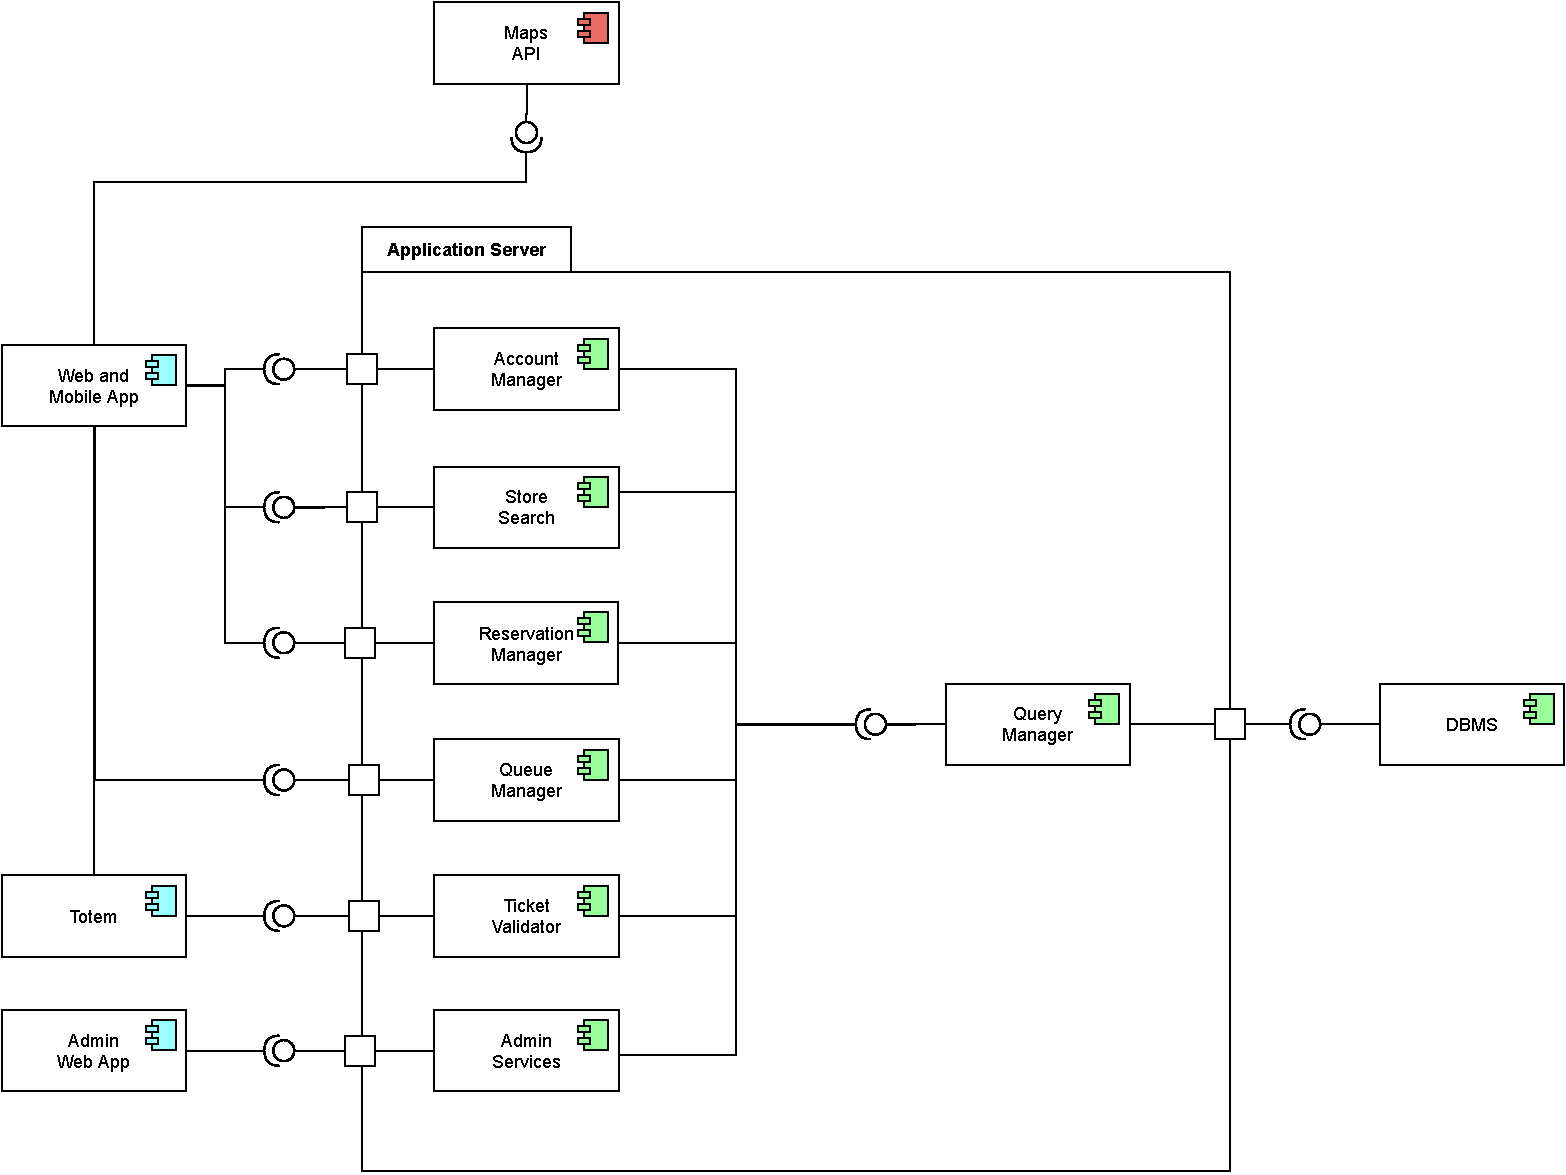
\includegraphics[width=\linewidth]{images/draw.io/component.pdf}
    \caption{Global Component Diagram of the System}
    \label{fig:component}
\end{figure}


\subsection{Deployment View}

\subsection{Runtime View}
% You can use sequence diagrams to describe the way components interact
% to accomplish specific tasks typically related to your use cases

\subsection{Component Interfaces}

\subsection{Selected Architectural Styles and Patterns}
%  Please explain which styles/patterns you used, why and how

\subsection{Other Design Decisions}
